% Preamble
\documentclass[a4paper, 12pt]{article}
\usepackage[margin=1in]{geometry} % Set margin
\usepackage{pdfpages} % Insert pdf pages
\usepackage{amssymb,amsmath,amsthm, amsfonts} % Math libraries

% Custom commands
\newcommand{\sub}[1]{\subsection{\underline{#1}}}
\newcommand{\subsub}[1]{\subsubsection{\underline{#1}}}
\newcommand{\R}{\ensuremath{\mathbb{R}}}
\newcommand{\F}{\ensuremath{\mathbb{F}}}
\newcommand{\N}{\ensuremath{\mathbb{N}}}
\newcommand{\Onef}{\ensuremath{1_{\F}}}
\newcommand{\Zerof}{\ensuremath{0_{\F}}}
\newcommand{\eqbcuz}[1]{\text{~$\stackrel{(#1)}{=}$~}}
\newcommand{\eq}[1]{\begin{align*}#1\end{align*}}
\newcommand{\eqn}[1]{\begin{align}#1\end{align}}
\newcommand{\set}[1]{\big{\{} #1 \big{\}}}
\renewcommand{\qed}{\hfill\(\qedsymbol\)}
\newtheorem{lemma}{Lemma}

% Begin Document %
\begin{document}

% Title Page
\begin{titlepage}
    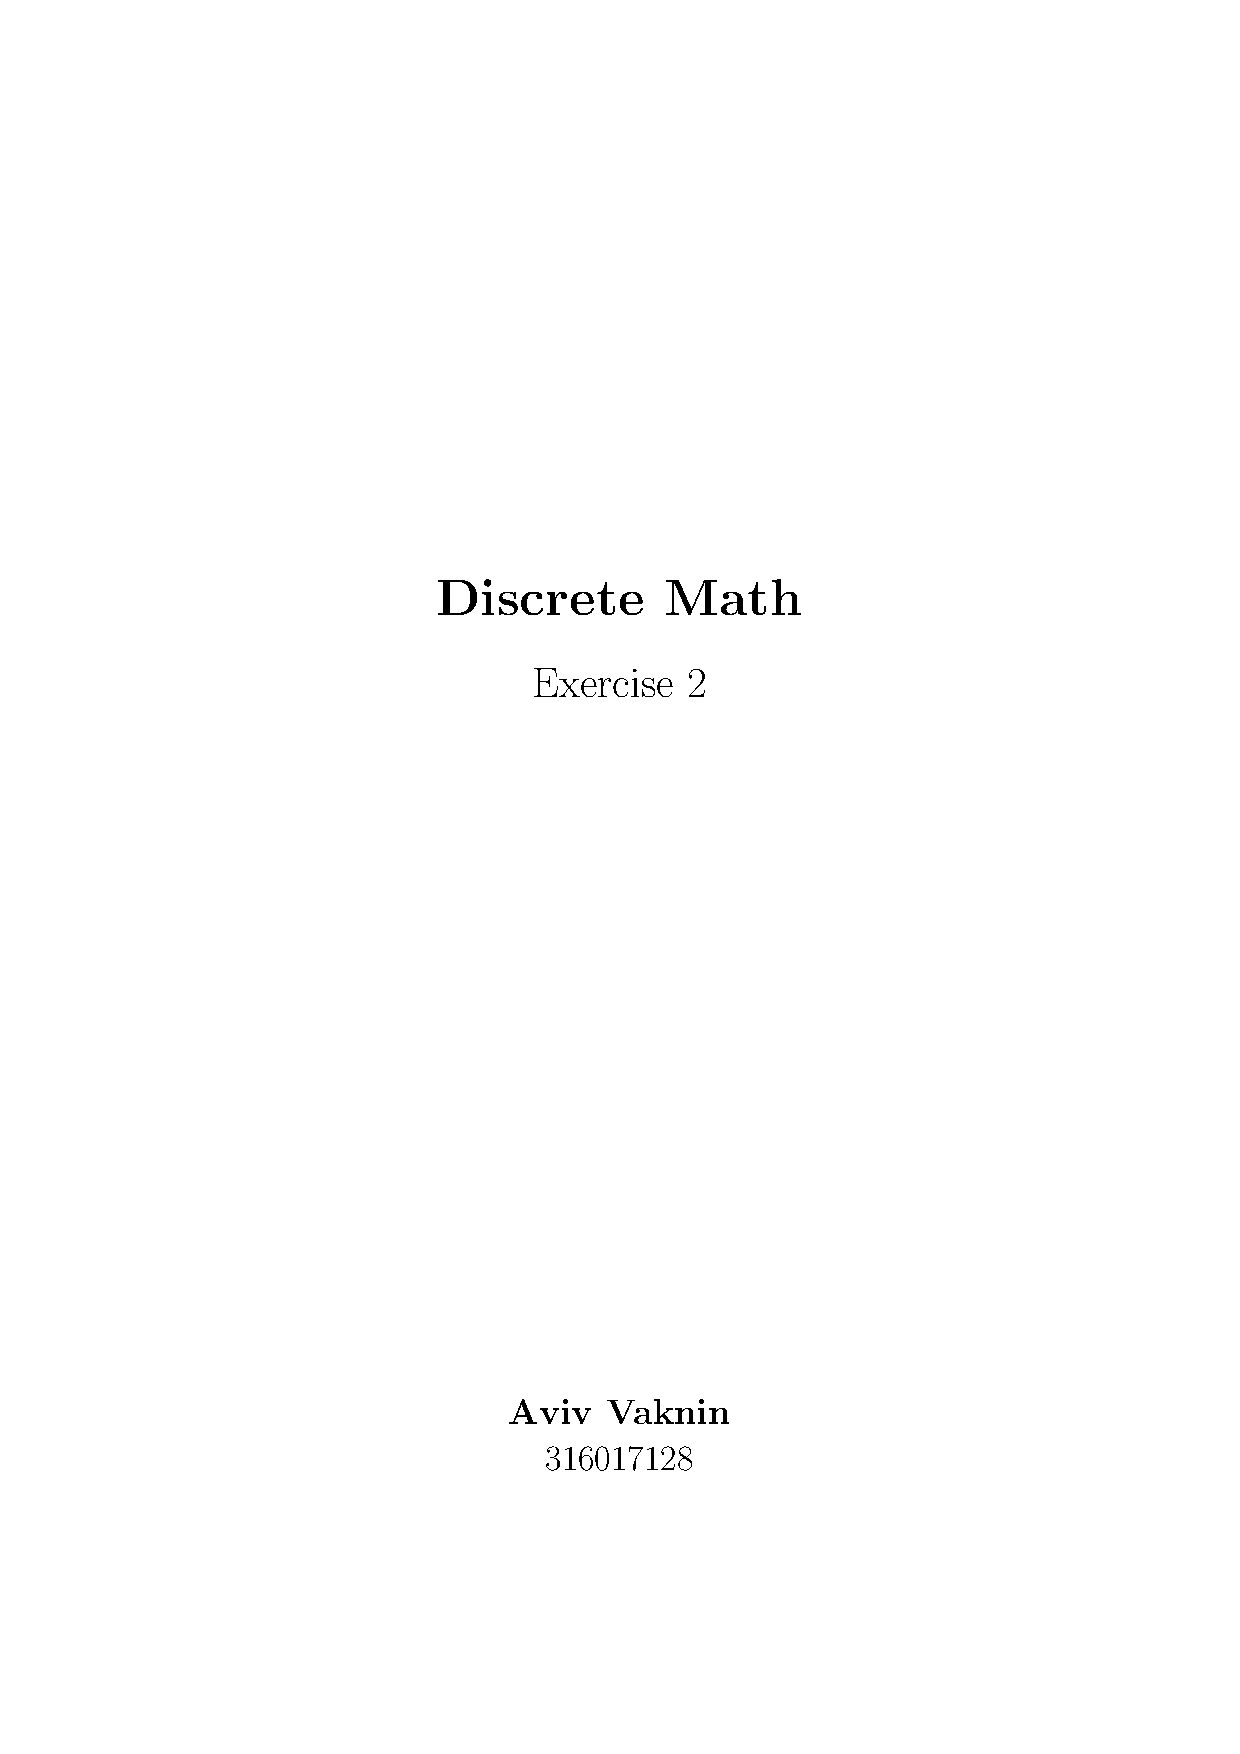
\includepdf{title.pdf}
\end{titlepage}

% 1
\section{}
\sub{$f(C_1\backslash{C_2})=f(C_1)\backslash{f(C_2)}$}
The statement is incorrect.\\
Let:
\eq{
    &A=\set{1,2,3}\\
    &B=\set{4,5,6}\\
    &f(1)=4\\
    &f(2)=5\\
    &f(3)=4\\
    &C_1=\set{1,2}\\
    &C_2=\set{2,3}
}
Therefore:
\eq{
    &f(C_1\backslash{C_2})=f(1)=4\\
    &f(C_1)\backslash{f(C_2)}=\set{4,5}\backslash\set{4,5}=\varnothing
}
Therefore, we can see that: \eq{f(C_1\backslash{C_2})\neq{f(C_1)\backslash{f(C_2)}}}
\sub{$f(C_1\cup{C_2})=f(C_1)\cup{f(C_2)}$}
In order to prove this identity, we'll need to show the following:
\eq{
    &f(C_1\cup{C_2})\subseteq{f(C_1)\cup{f(C_2)}}\\
    &{f(C_1)\cup{f(C_2)}\subseteq{f(C_1\cup{C_2})}}
}
\subsub{$f(C_1\cup{C_2})\subseteq{f(C_1)\cup{f(C_2)}}$}
Let $y\in f(C_1\cup{C_2})$.\\
Therefore, there exists $x\in{C_1\cup{C_2}}$ such that $f(x)=y$.\\
Hence, there are two possibilities, $x\in{C_1}$ or $x\in{C_2}$.\\
If $x\in{C_1}$, then $y\in f({C_1})$, and similarly, if $x\in{C_2}$, then $y\in f({C_2})$.\\
Therefore, $y\in f({C_1})$ or $y\in f({C_2})$, or formally:
\eq{y\in f({C_1})\cup f({C_2})}

\subsub{${f(C_1)\cup{f(C_2)}\subseteq{f(C_1\cup{C_2})}}$}
Let $y\in f(C_1)\cup f({C_2})$.\\
If $y\in f(C_1)$, then there exists an $x\in{C_1}$ such that $f(x)=y$.\\
If $x\in{C_1}$, then $x\in{C_1}\cup{C_2}$, and therefore $f(x)=y$ still stands.\\
Therefore:
\eq{y\in f({C_1}\cup{C_2})}
\qed\pagebreak

% 2
\section{}
\sub{}
The statement is true.
First, let's look at: $f(C)\cap D$\\
Let: \eq{y\in f(C)\cap D}
Therefore:
\eqn{
    &y\in f(c)\\
    &y\in D
}
Now, let's look at: $f(C\cap f^{-1}(D))$\\
Let: \eq{x\in C\cap f^{-1}(D)}
Therefore: \eqn{&x\in{C}\\&x\in{f^{-1}(D)}}
If we apply $f$ on 3 and 4, we'll return to 1 and 2, accordingly.

\sub{}
The statement is incorrect, here's a counter example:
\eq{
    &A=\set{1}\\
    &B=\set{2,3}\\
    &C=A=\set{1}\\
    &D=\set{2}\\
    &f(1)=3\\
}
Now, we can see:
\eq{
    &f(C)\cup{D}=\set{2,3}\\
    &f(C\cup{f^{-1}(D))}=f(\set{1}\cup\set{})=f(\set{1})=f(1)=3\\
    &\set{2,3}\neq\set{3}
}
\qed
\pagebreak

% 3
\section{}
It is given that $g\circ{f}$ is surjective, therefore:
\eq{
    (\forall{y}\in{C})~(\exists{x}\in{A})~g(f(x))=y
}
We want to show that $g$ is surjective, that is:
\eq{
    (\forall{y}\in{C})~(\exists{x}\in{B})~g(x)=y
}
Because \textit{f} is defined as:
\eq{
    f:A\longrightarrow{B}
}
We can read $g\circ{f}$ surjection as: "\textit{f} outputs \textit{g}'s input, and then every output of \textit{g} is surjective".\\
Therefore, we can conclude that if $g\circ{f}$ is surjective, \textit{g} \textbf{must} be surjective as well.

%4
\section{}
\sub{}
The statement is incorrect.\\
Let:
\eq{
    &A=\set{1,2}\\
    &B=\set{3,4}\\
    &C=\set{5}\\
    &f(1)=3\\
    &f(2)=3\\
    &g(1)=4\\
    &g(2)=4\\
    &h(3)=5\\
    &h(4)=5
}
Therefore, we can see that h is \textbf{surjective}, $h\circ{f}=h\circ{g}$, but $g\neq{f}$.
\qed
\sub{}
The statement is correct, let's show it.\\
it is given that $h\circ{f}=h\circ{g}$, therefore:
\eq{
    \forall{x}\in{A}~~h(f(x))=h(g(x))
}
However, because it is given that h is \textbf{injective}, we can conclude that:
\eq{g(x)=f(x)}
And therefore:
\eq{g=f}
\qed

% 5
\section{}
\sub{Compute $g\circ{f}$}
\eq{
    h_1=\bigg{(}
    \begin{matrix}
        1&2&3&4&5&6&7\\
        3&2&6&4&1&7&5
    \end{matrix}
    \bigg{)}
}
\sub{Compute $f\circ{g}$}
\eq{
    h_2=\bigg{(}
    \begin{matrix}
        1&2&3&4&5&6&7\\
        3&2&7&1&5&4&6
    \end{matrix}
    \bigg{)}
}
\sub{Find the order of $h_1$ and $h_2$}
First, we'll factor $h_1$ and $h_2$:
\eq{
    h_1=(13675)(2)(4)\\
    h_2=(13764)(2)(5)
}
Therefore, the order of $h_1$ and $h_2$ is 5.
\sub{Find the permutation $h_1^{5781}$ and $h_2^{5782}$}
\subsub{$h_1^{5781}$}
We can see that: \eq{5781~mod~5=1}
Therefore: \eq{
    h_1^{5781}=h_1^1=h_1=\bigg{(}
    \begin{matrix}
        1&2&3&4&5&6&7\\
        3&2&6&4&1&7&5
    \end{matrix}
    \bigg{)}
}
\subsub{$h_2^{5782}$}
We can see that: \eq{5782~mod~5=2}
Therefore: \eq{
    h_2^{5782}=h_2^2=\bigg{(}
    \begin{matrix}
        1&2&3&4&5&6&7\\
        7&2&6&3&5&1&4
    \end{matrix}
    \bigg{)}
}

\end{document}